Robot Operating System (ROS) to framework do pisania oprogramowania robotów.
Jest to zbiór narzędzi, bibliotek i~konwencji, które mają na celu uproszczenie
zadania tworzenia złożonych zachowań robotów na wielu różnych platformach
robotyki.

Architektura środowiska uruchomieniowego ROS to sieć procesów
\textit{peer-to-peer} (potencjalnie rozproszona na komputerach), które są luźno
połączone za pomocą infrastruktury komunikacyjnej ROS.

\textbf{Peer-to-peer (P2P)} to model komunikacji, w~którym każda ze stron ma te
same uprawnienia i każda ze stron może zainicjować sesję komunikacyjną.
ROS implementuje kilka różnych stylów komunikacji, w~tym synchroniczną
komunikację w stylu RPC za pośrednictwem usług, asynchroniczne przesyłanie
danych do tematów i przechowywanie danych na serwerze parametrów.

\textbf{RPC (ang. \textit{remote procedure call})} polega na tym ,że gdy
program komputerowy powoduje wykonanie procedury (podprogramu), w~innej
przestrzeni adresowej (zwykle na innym komputerze w sieci współdzielonej),
która jest kodowana tak, jakby była normalnym (lokalnym) wywołaniem procedury,
bez programisty jawnie kodującego szczegóły dotyczące zdalnej interakcji.

\section{Komunikacja publish-subscribe}
W architekturze oprogramowania na platformie ROS, komunikacja odbywa się
zgodnie protokołem przesyłania wiadomości \textbf{publish-subscribe} (rys.
\ref{fig:pubsub}), realizujące połączenie pomiędzy poszczególnymi
\textbf{węzłami}.
Protokół publish-subscribe, polega na tym, że węzły wysyłające wiadomości,
nazywane \textbf{węzłami publikującymi}, nie określają
do jakiego konkretnego odbiorcy, nazywanego \textbf{węzłem subskrybującym}, ma
dana wiadomość trafić.
W zamian, kategoryzują wysyłane wiadomości na klasy, które z~kolei nazywamy
\textbf{tematami}, bez żadnej informacji do jakiego,
jeżeli do jakiegokolwiek węzła, ma ona trafić.
Cała komunikacja odbywa się dzięki serwerowi (nazywanemu \textbf{ROS Master}),
który umożliwia węzłowi subskrybującemu zidentyfikowanie źródła danych będących
przedmiotem zainteresowania.
Ten paradygmat daje możliwość istnienia wielu jednoczesnych
węzłów publikujących i~subskrybujących.
Jeden węzeł publikujący może publikować dane do wielu węzłów subskrybujących
lub zasubskrybować się u jednego z innych wydawców w~bieżącym systemie.

\begin{figure}
  \centering
  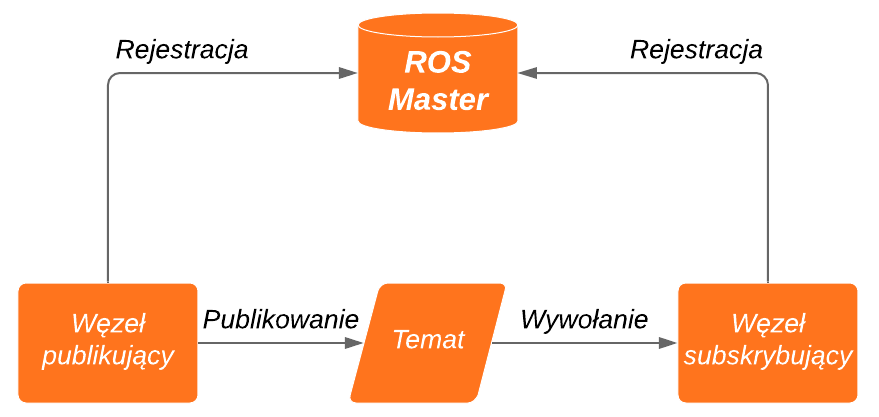
\includegraphics[width=105mm]{graphics/ROSflow.png}
\caption{Schemat przepływowy danych w protokole publish-subscribe, na
platformie ROS}
  \label{fig:pubsub}
\end{figure}

W~ROS węzeł jest jednostką lub procesem, który wykonuje pewną formę obliczeń
i/lub przetwarzania i akwizycji sygnałów.
Urządzenia i~systemy wykorzystywane przez pojazd, który jest omawiany
w~niniejszym projekcie, można przedstawić za pomocą węzłów.
Na przykład, węzeł na dane enkodera, węzeł dla urządzenia LiDAR,
węzeł do autonomicznej jazdy (w tym nawigacja, planowanie trasy, unikanie
przeszkód), węzeł do wizualizacji.
Węzły porozumiewają się ze sobą za pomocą struktur danych (określane jako typy
wiadomości) które składają się z~wymaganych pól będących typu liczba całkowita,
liczba zmiennoprzecinkowa, wartość logiczna czy też obiekt pewnej klasy.
Jeśli węzeł chce się komunikować z~innym węzłem, opublikuje wiadomość
o~określonej strukturze do tematu, a~inny węzeł zasubskrybuje ten temat
(oczekując określonego typu wiadomości i~pola) i~gromadząc wymagane dane.
Przy każdej dostarczonej wiadomości, w~węźle subskrybującym aktywowane jest
wywołanie (ang. \textit{callback}), w~którym zdefiniowane są, dalsze czynności
powiązane z~tą wiadomością np. przetworzenie w określony sposób i~przekazanie
do kolejnego węzła.

\section{Model URDF}
\textbf{Unified Robot Description Format (URDF)} to specyfikacja XML opisująca
robota. Roboty formacie URDF są reprezentowane w strukturze drzewa, które
przedstawia stworzoną hierarchię połączeń pomiędzy poszczególnymi członami
modelu. Specyfikacja zakłada, że robot składa się ze sztywnych elementów
połączonych ze sobą. Specyfikacja obejmuje kinematyczny i dynamiczny opis,
wizualną reprezentację oraz model zderzeniowy robota.

Na poziomie implementacji plik URDF jest po prostu plikiem tekstowym
zawierającym znaczniki XML: określone słowa kluczowe, które ROS rozpoznaje jako
część URDF.

Niektóre ze znaczników XML odnoszą się do innych plików lub modeli 3D części
robotów, co pozwala korzystać z plików zewnętrznych w celu szybkiego włączenia
szczegółowego kształtu wraz z kolorystyką.

Opis robota składa się z zestawu członów(ang. \textit{links}) i~zestawu
elementów łączących ze sobą człony(\textit{ang. joints}).

\begin{figure}[h]
\centering
\subfloat[Złącze
(\textit{joint})]{{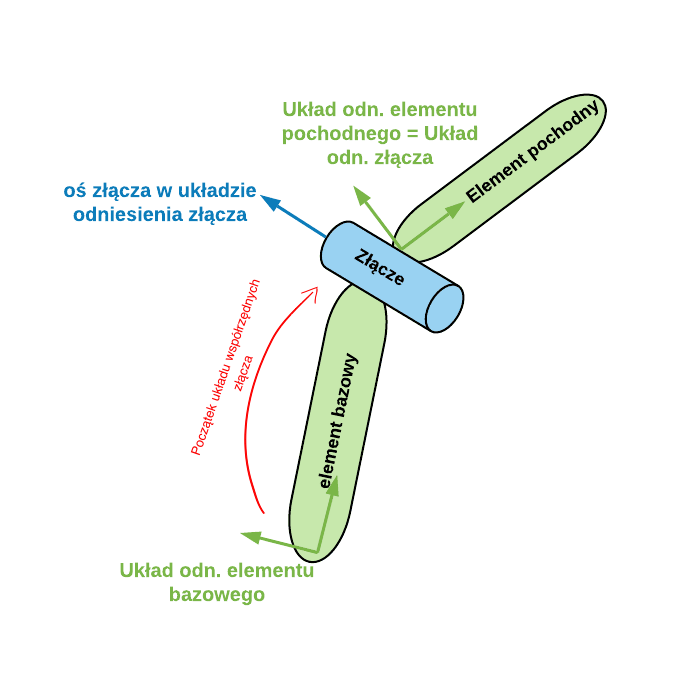
\includegraphics[width=7cm]{graphics/joint2.png} }}%
\qquad
\subfloat[Człon robota
(\textit{link})]{{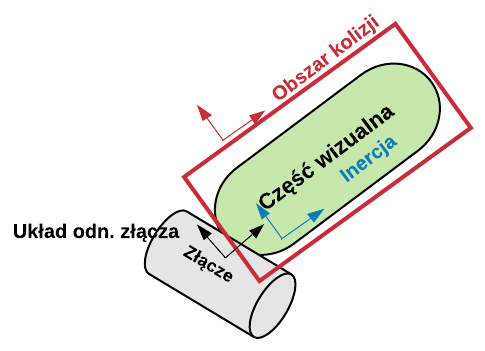
\includegraphics[width=7cm]{graphics/link.png} }}%
\caption{Elementy struktury opisu robota w formacie URDF.}%
\label{fig:linkjoint}
\end{figure}

\textbf{Człon robota} (\textit{link}) opisuje sztywny korpus o bezwładności,
cechach wizualnych i właściwościach kolizji.

\textbf{Złącze}(\textit{joint}) opisuje kinematykę i dynamikę złącza,
umiejscowienie połączenia, element bazowy oraz element pochodny, między którymi
stworzone jest dane złącze.

\section{Środowisko symulacyjne}
Symulacja robota pomaga obniżyć całkowity koszt integracji. Dzieje się tak
głównie dzięki możliwości symulowania aplikacji w świecie rzeczywistym bez
fizycznych kosztów związanych z tym faktem. Symulacja robota również zmniejsza,
a często nawet eliminuje potrzebę wprowadzania zmian w systemie po jego
zainstalowaniu, ponieważ już udowodniono, że jego procesy działają.

Spośród dostępnych otwarto-źródłowych symulatorów 3D, w celu zasymulowania 
pracy robota oraz pomiarów ze skanera LIDAR, wybrano symulator \textit{Gazebo}.
Głównym powodem tego wyboru jest kompatybilność z wykorzystywaną platformą ROS.
Oprócz tego, Gazebo zapewnia wysokowydajne silniki fizyki, realistyczne
renderowanie środowisk, w tym wysokiej jakości oświetlenie, cienie i tekstury.

\begin{figure}
  \centering
  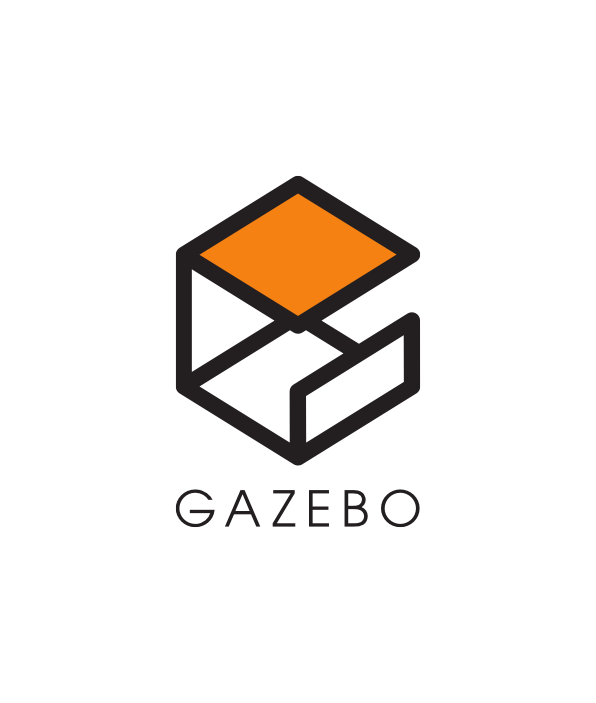
\includegraphics[width=40mm]{graphics/gazebologo.png}
  \caption{Logo symulatora Gazebo 3D}
  \label{fig:gazebologo}
\end{figure}

Istotną cechą tego symulatora jest możliwość generowania danych czujników,
opcjonalnie z szumem, ze skanerów laserowych, kamer 2D/3D, czujników w~stylu
Kinect, czujników kontaktowych, siły momentu obrotowego i innych.

Obslugiwany przez symulator ROS format SDF opisuje obiekty i~środowisko dla
symulacji, wizualizacji i~sterowania robotem.
Pozwala dokładnie opisać
wszystkie aspekty robota, a~w~razie potrzeby, w~łatwy sposób można go
przekonwertować na format URDF.
Oprócz możliwości tworzenia własnych robotów Gazebo zapewnia kilka modeli,
gotowych do przetestowania.

\section{Symulacja omni robota}
Na poniższym obrazku znajduje się wizualizacja omni robota, który został
stworzony dla celów realizacji projektu.
Początkowo poszczególne części
zostały zaprojektowane jako siatka graficzna, wykorzystując do tego specjalne
programy graficzne, a~następnie wszystkie stworzone elementy robota zostały
zintegrowane ze sobą w formacie URDF.

Wykorzystując wspomniany format (URDF), stworzono odpowiedni model, który
opisuje również momenty bezwładności poszczególnych elementów, co pozwala na
odwzorowanie tego, jak zachowałby się podobny robot w świecie rzeczywistym.

Na robocie znajduje się platforma, na której w dalszym etapie tworzenia modelu,
został zamontowany skaner laserowy LiDAR.

\begin{figure}
  \centering
  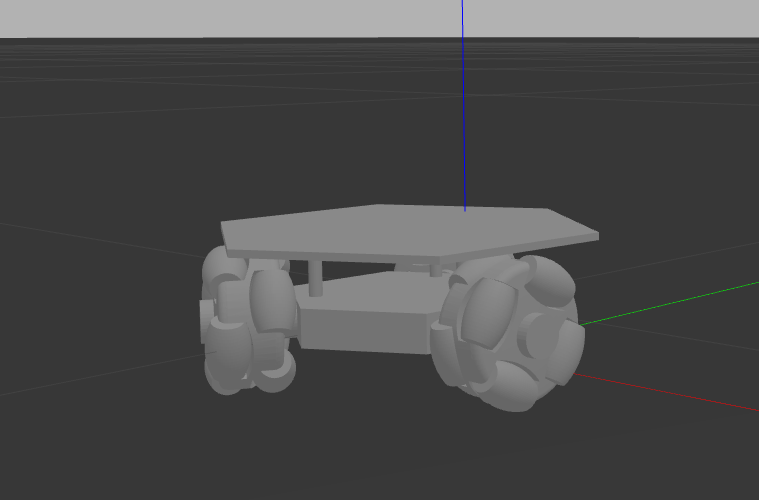
\includegraphics[width=140mm]{graphics/robot.png}
  \caption{Symulacja omni-robota}
  \label{fig:forklift}
\end{figure}
\newpage
